\documentclass[
    10pt,
    aspectratio=169,
    xcolor={dvipsnames},
    spanish,
    % handout,
    % notes=only,
    % notes,
    ]{beamer}

% BEAMER SETTINGS
\setbeamerfont{section in toc}{size=\normalsize, shape=\bfseries}
\mode<presentation>{
    \usetheme{Antibes}
    \setbeamercovered{transparent}
    \usecolortheme{rose}
    \setbeamertemplate{navigation symbols}{}
    }
\useoutertheme{infolines}

% PACKAGES
\usepackage[spanish]{babel}  % uncomment for Spanish support
\usepackage{tikz,pgfplots}
\pgfplotsset{compat=1.13}
\usetikzlibrary{calc}

\usepackage{graphicx}
\graphicspath{{figures}}
\usepackage{booktabs}
\usepackage{upgreek}
\usepackage{commath}
\usepackage{amsmath,amsthm,amssymb,mathtools,mathrsfs}
\usepackage{cancel}
\usepackage{fontawesome5}
\usepackage{enumerate}
\usepackage{tensor}
\usepackage[font=footnotesize]{caption}
\usepackage{wasysym}

\usepackage[skins,theorems]{tcolorbox}
\tcbset{
    highlight math style={
        enhanced,
        coltext=black,
        colframe=black,
        colback=lightgray,
        arc=0pt,
        boxrule=.5pt
        }
}

% REFERENCES AND OTHERS
\usepackage{aas_macros}
\usepackage{natbib}
\bibpunct{(}{)}{;}{a}{}{,}

\renewcommand{\figurename}{Fig.}

\usepackage{hyperref}
\hypersetup{
    % bookmarks=true,
    unicode=true,
    pdftoolbar=true,
    pdfmenubar=true,
    pdffitwindow=false,
    pdfstartview={FitH},
    pdftitle={Presentation},
    pdfauthor={Tomas Cassanelli},
    pdfcreator={Tomas Cassanelli},
    pdfnewwindow=true,
    colorlinks=true,
    linkcolor=RoyalBlue,
    citecolor=RoyalBlue,
    urlcolor=RoyalBlue
    }

\title[EL3103]{\bfseries Transistores}
\subtitle{Teoría y aplicación}
\author[San Martín, Rabin, Gutierrez]{Javier San Martín, Benjamín Rabin, Nicolás Gutierrez}
\institute[UChile]{Departmento de Ingeniería Eléctrica \\ Universidad de Chile}

\date{\today}

\begin{document}

\begin{frame}
  \titlepage
  \centering
\end{frame}

\begin{frame}
  \frametitle{Contenidos}
  \centering
  \begin{columns}
    \begin{column}{0.4\textwidth}
      \tableofcontents
    \end{column}
    \begin{column}{0.5\textwidth}
      \begin{figure}
        \centering
        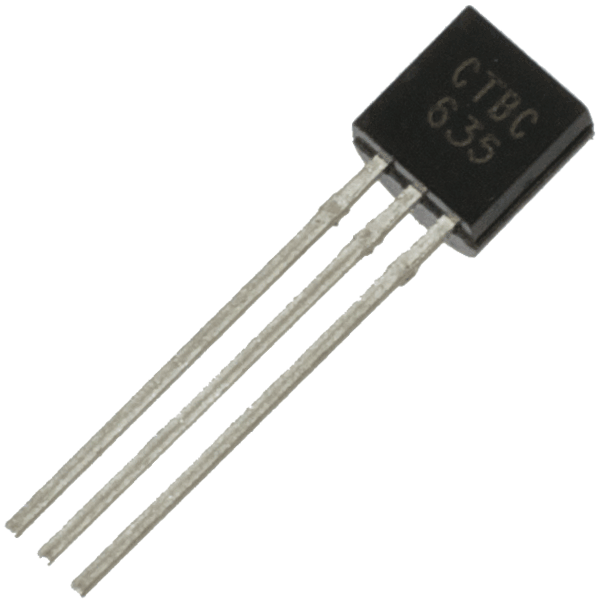
\includegraphics[width=0.5\textwidth]{figures/Bc635-transistor.png}
        \caption{Transistor BJT NPN BC635}
      \end{figure}
    \end{column}
  \end{columns}  
\end{frame}

\section{Introducción}

\begin{frame}
    \frametitle{Introducción}
    \centering
    \begin{columns}
        \begin{column}{0.4\textwidth}
            \begin{itemize}
                \item ¿Qué es un transistor?
                \item ¿Para qué se usa?
            \end{itemize}  
        \end{column}
        \begin{column}{0.5\textwidth}
            \begin{figure}
                \centering
                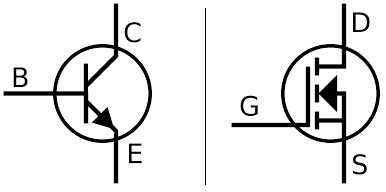
\includegraphics[width=0.8\textwidth]{figures/BJT-vs-FET.png}
                \caption{Simbología transistores, BJT (izquierda), MOSFET (derecha)}
            \end{figure}
        \end{column}
    \end{columns}
\end{frame}

\section{Historia}

\begin{frame}
    \frametitle{Historia e invención}
    \centering
    \begin{columns}
        \begin{column}{0.5\textwidth}
            \begin{figure}
                \centering
                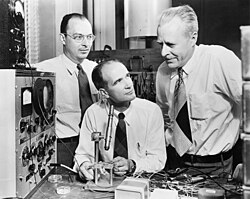
\includegraphics[width=0.7\linewidth]{figures/Bardeen_Shockley_Brattain_1948.JPG}
                \caption{John Bardeen, William Shockley y Walter Brattain en Bell Labs en 1948}
            \end{figure}
        \end{column}
        \begin{column}{0.5\textwidth}
            \begin{figure}
                \centering
                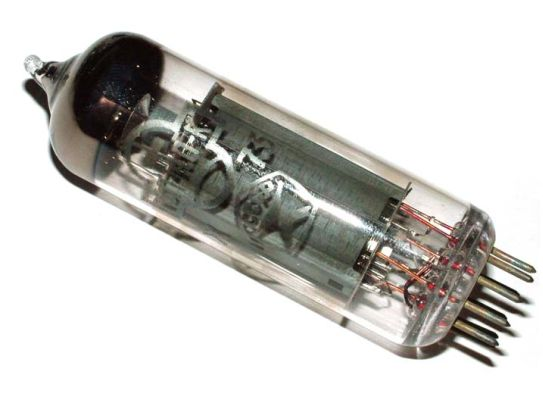
\includegraphics[width=0.7\linewidth]{figures/Tubo_de_vacio.jpg}
                \caption{Tubo de Vacío}
            \end{figure}
        \end{column}
    \end{columns}
\end{frame}

\section{Semicondutores}

\begin{frame}
    \frametitle{Semiconductores}
    \begin{columns}
        \begin{column}{0.35\textwidth}
            \begin{itemize}
                \item Materiales intrínsecos
            \end{itemize}
            \begin{figure}
                \centering
                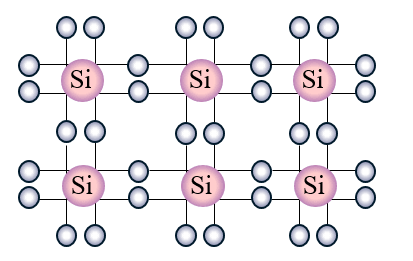
\includegraphics[width=0.7\linewidth]{figures/silicon.png}
                \caption{Átomos de silicio formando una estructura cristalina}
            \end{figure}
        \end{column}
        \begin{column}{0.65\textwidth}
            \begin{figure}
                \centering
                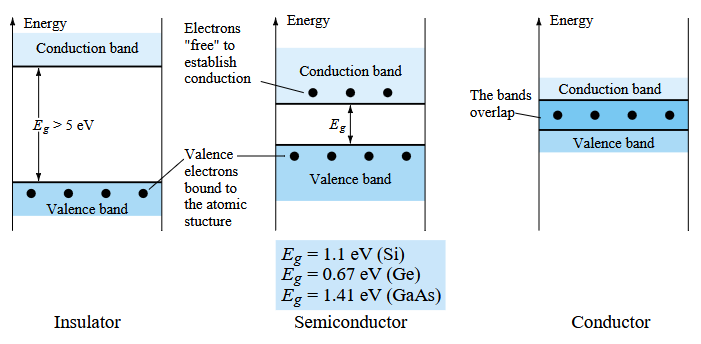
\includegraphics[width=1\linewidth]{figures/bandas de conduccion y valencia.png}
                \caption{Bandas de conducción y valencia para distintos materiales}
            \end{figure}
        \end{column}
    \end{columns}
\end{frame}

\begin{frame}
    \frametitle{Doping}
    \begin{columns}
        \begin{column}{0.4\textwidth}
            \begin{itemize}
                \item Materiales tipo n
                \item Materiales tipo p
                \item Electrones vs huecos
                \item Movimiento de cargas
            \end{itemize}
        \end{column}
        \begin{column}{0.5\textwidth}
            \begin{figure}
                \centering
                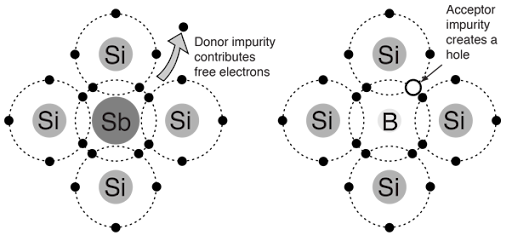
\includegraphics[width=0.9\linewidth]{figures/silicon doping.png}
                \caption{Doping de silicio utilizando estroncio (tipo n) y boro (tipo p)}
            \end{figure}
        \end{column}
    \end{columns}
\end{frame}

\begin{frame}
    \frametitle{¿Qué ocurre al unir n y p?}
    \begin{columns}
        \begin{column}{0.4\textwidth}
            \begin{itemize}
                \item Diodo
                \item Región de agotamiento
                \item Equilibrio
            \end{itemize}
        \end{column}
        \begin{column}{0.6\textwidth}
            \begin{figure}
                \centering
                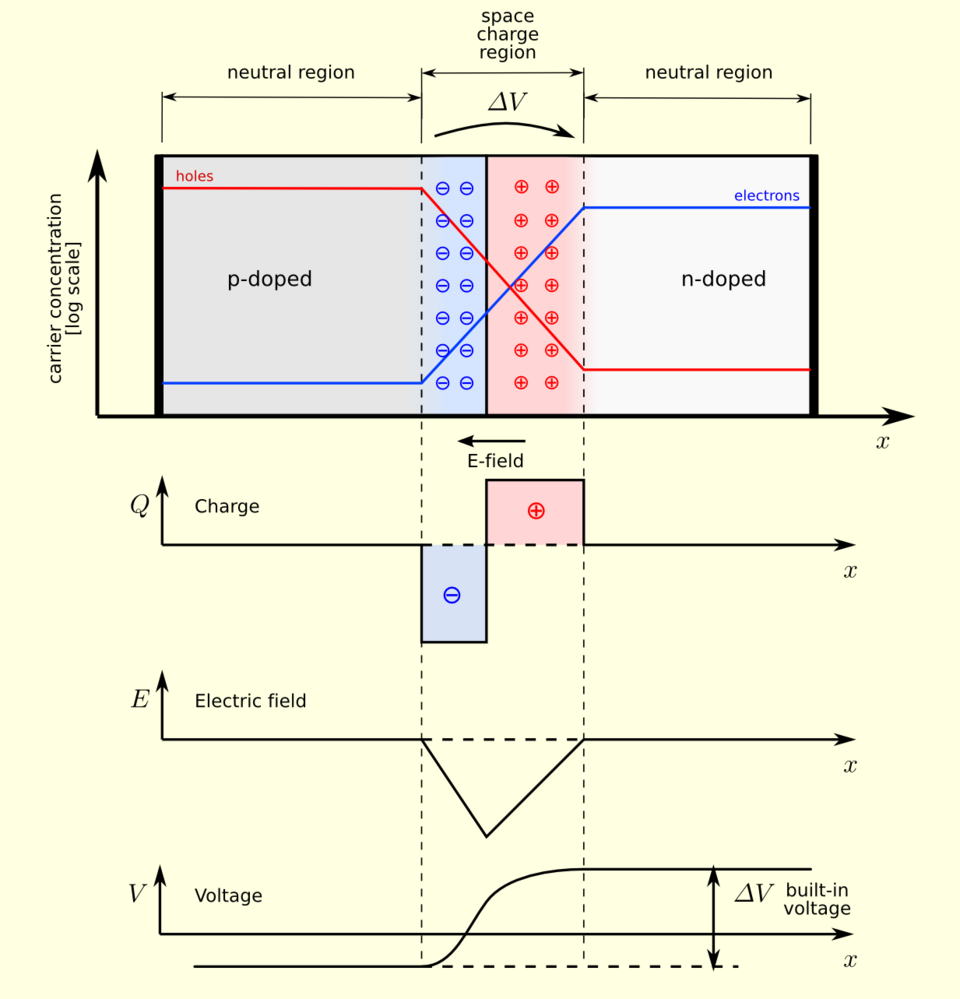
\includegraphics[width=0.65\linewidth]{figures/Pn-junction-equilibrium-graphs.png}
                \caption{Equilibrio de la unión n-p}
            \end{figure}
        \end{column}
    \end{columns}
\end{frame}

\begin{frame}
    \frametitle{¿Qué ocurre al unir n y p?}
    \begin{itemize}
        \item ¿Qué ocurre al aplicar voltaje?
    \end{itemize}
    \begin{figure}
        \centering
        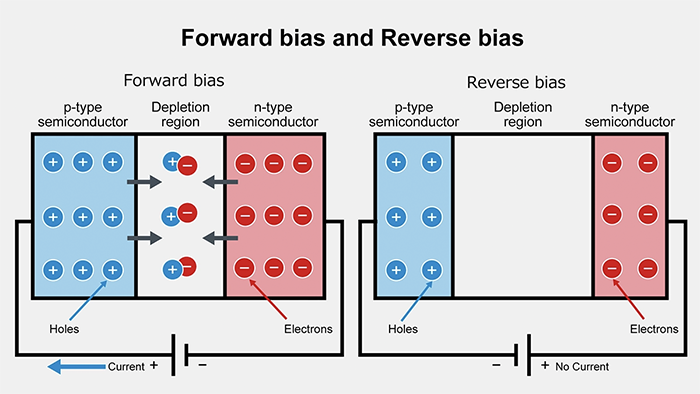
\includegraphics[width=0.6\linewidth]{figures/04-forward-bias-reverse-bias-en.png}
        \caption{Efectos de aplicar voltaje sobre la unión n-p}
    \end{figure}
\end{frame}

\begin{frame}
    \frametitle{¿Qué ocurre al unir n y p?}
    \begin{columns}
        \begin{column}{0.5\textwidth}
            \begin{figure}
                \centering
                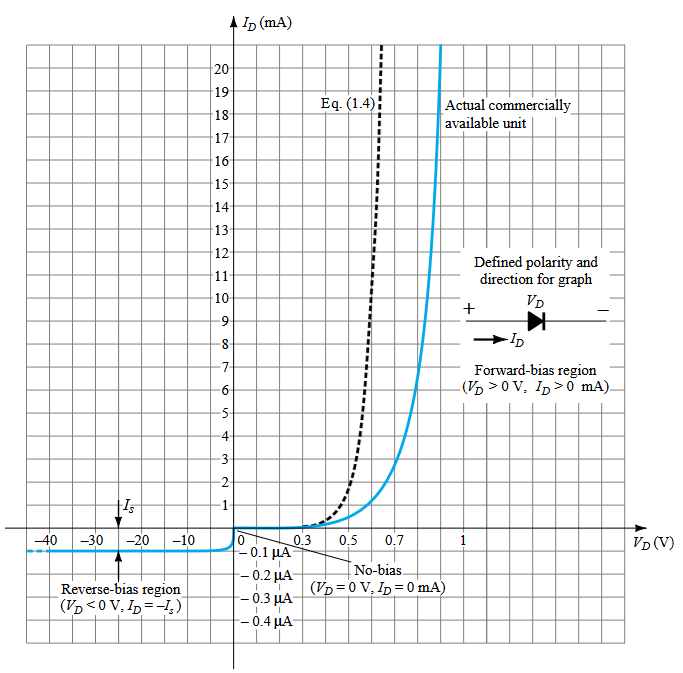
\includegraphics[width=0.8\linewidth]{figures/diode-characteristics.png}
                \caption{Curva característica de un diodo}
            \end{figure}
        \end{column}
        \begin{column}{0.5\textwidth}
            \begin{itemize}
                \item Característica I-V de un diodo
                \begin{equation*}
                    I_D=I_s(e^{kV_D/T_K}-1)
                \end{equation*}
                \item Resistencia estática de un diodo
                \begin{equation*}
                    R_D=\frac{V_D}{I_D}
                \end{equation*}
            \end{itemize}
        \end{column}
    \end{columns}
\end{frame}

\section{Transistor de unión bipolar (BJT)}

\begin{frame}
    \frametitle{Transistor de unión bipolar (BJT)}
    \begin{columns}
        \begin{column}{0.4\textwidth}
            \begin{itemize}
                \item Dos uniones p-n
                \item Base, emisor y colector
                \item PNP y NPN
                \item Usa electrones y huecos como portadores de carga
            \end{itemize}
        \end{column}
        \begin{column}{0.6\textwidth}
            \begin{figure}
                \centering
                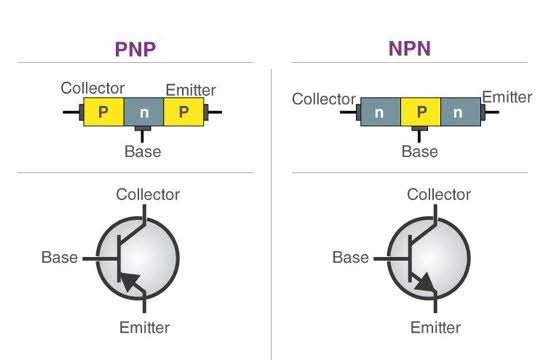
\includegraphics[width=0.9\linewidth]{figures/bjt npn vs pnp.jpg}
                \caption{Transistores PNP y NPN}
            \end{figure}
        \end{column}
    \end{columns}
\end{frame}

\begin{frame}
    \frametitle{Eficiencia y ganancia}
    Por la ley de corrientes de Kirchhoff, la corriente que entra al emisor es igual a la suma de las corrientes que salen por el colector y la base:
    \begin{equation*}
        I_E = I_C + I_B
    \end{equation*}
    La proporcion de la corriente del colector repecto a la corriente del emisor se conoce como $\alpha$:
    \begin{equation*}
        \alpha = \frac{I_C}{I_E}
    \end{equation*}
    La proporcion de la corriente del colector respecto a la corriente de la base se conoce como $\beta$:
    \begin{equation*}
        \beta = \frac{I_C}{I_B}
    \end{equation*}
    La relación entre $\alpha$ y $\beta$ es:
    \begin{equation*}
        \beta = \frac{\alpha}{1 - \alpha}
    \end{equation*}
\end{frame}

\begin{frame}
    \frametitle{Regiones operativas}
    \begin{columns}
        \begin{column}{0.4\textwidth}
            \begin{itemize}
                \item Polarización de las uniones
                \item Región activa directa
                \begin{itemize}
                    \item Región activa inversa
                \end{itemize}
                \item Región de corte
                \item Región de saturación
            \end{itemize}
        \end{column}
        \begin{column}{0.6\textwidth}
            \begin{figure}
                \centering
                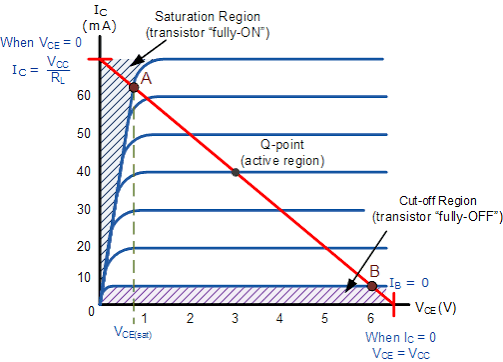
\includegraphics[width=0.8\linewidth]{figures/regiones de operacion bjt.png}
                \caption{Regiones operativas BJT}
            \end{figure}
        \end{column}
    \end{columns}
\end{frame}

\begin{frame}
    \frametitle{Regiones operativas}
    \begin{table}[t]
        \centering
        \begin{tabular}{ccccc}
            \toprule
            \textbf{Junction type} & \textbf{Applied voltages} & \multicolumn{2}{c}{\textbf{Junction bias}} & \textbf{Mode} \\
            & & \textbf{B--E} & \textbf{B--C} & \\ \midrule
            NPN & $E < B < C$ & Forward & Reverse & Forward-active \\
            NPN & $E < B > C$ & Forward & Forward & Saturation \\
            NPN & $E > B < C$ & Reverse & Reverse & Cut-off \\
            NPN & $E > B > C$ & Reverse & Forward & Reverse-active \\ \midrule
            PNP & $E < B < C$ & Reverse & Forward & Reverse-active \\
            PNP & $E < B > C$ & Reverse & Reverse & Cut-off \\
            PNP & $E > B < C$ & Forward & Forward & Saturation \\
            PNP & $E > B > C$ & Forward & Reverse & Forward-active \\
            \bottomrule
        \end{tabular}
        \caption{Tabla de Regiones Operativas}
    \end{table}
\end{frame}

\begin{frame}
    \frametitle{Configuraciones topológicas}
    \begin{itemize}
        \item Terminal común a la entrada y salida
    \end{itemize}
    \begin{figure}
        \centering
        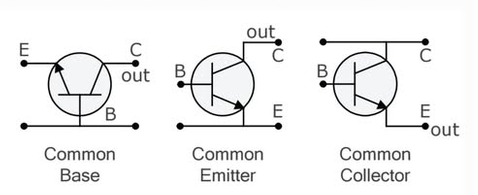
\includegraphics[width=0.8\linewidth]{figures/bjt topology.png}
        \caption{Configuraciones topológicas del BJT}
    \end{figure}
\end{frame}

\begin{frame}
    \frametitle{Emisor común}
    \begin{columns}
        \begin{column}{0.4\textwidth}
            \begin{itemize}
                \item \textbf{Ganancia de voltaje ($A_v$):} Alta.
                \item \textbf{Ganancia de corriente ($A_i$):} Alta ($\beta$).
                \item \textbf{Impedancias:} Entrada moderada (unos cuantos k$\Omega$), salida moderada-alta.
                \item \textbf{Fase:} Invierete la señal $180^\circ$.
            \end{itemize}
        \end{column}
        \begin{column}{0.6\textwidth}
            \begin{figure}
                \centering
                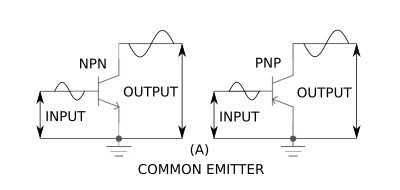
\includegraphics[width=0.8\linewidth]{figures/transistor-configurationse.jpg}
                \caption{Configuración de emisor común}
            \end{figure}
        \end{column}
    \end{columns}
\end{frame}

\begin{frame}
    \frametitle{Colector común}
    \begin{columns}
        \begin{column}{0.4\textwidth}
            \begin{itemize}
                \item \textbf{Ganancia de voltaje ($A_v$):} $\approx 1$, nunca mayor a $1$.
                \item \textbf{Ganancia de corriente ($A_i$):} Alta.
                \item \textbf{Impedancias:} Entrada muy alta, salida muy baja.
                \item \textbf{Fase:} En fase ($0^\circ$).
            \end{itemize}
        \end{column}
        \begin{column}{0.6\textwidth}
            \begin{figure}
                \centering
                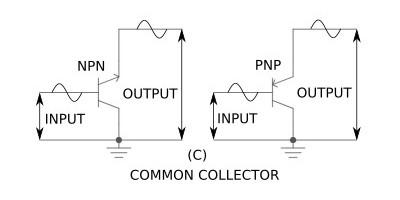
\includegraphics[width=0.8\linewidth]{figures/transistor-configurationsc.jpg}
                \caption{Configuración de colector común}
            \end{figure}
        \end{column}
    \end{columns}
\end{frame}

\begin{frame}
    \frametitle{Base común}
    \begin{columns}
        \begin{column}{0.4\textwidth}
            \begin{itemize}
                \item \textbf{Ganancia de voltaje ($A_v$):} Alta.
                \item \textbf{Ganancia de corriente ($A_i$):} $\approx 1$ ($\alpha$).
                \item \textbf{Impedancias:} Entrada muy baja, salida alta.
                \item \textbf{Fase:} En fase ($0^\circ$).
            \end{itemize}
        \end{column}
        \begin{column}{0.6\textwidth}
            \begin{figure}
                \centering
                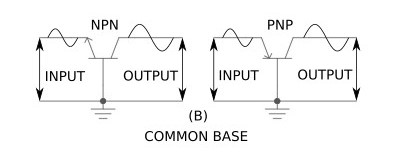
\includegraphics[width=0.8\linewidth]{figures/transistor-configurationsb.jpg}
                \caption{Configuración de base común}
            \end{figure}
        \end{column}
    \end{columns}
\end{frame}

\begin{frame}
    \frametitle{Configuraciones topológicas}
    \begin{table}[htpb]
        \centering
        \begin{tabular}{llll}
            \toprule
            \textbf{Característica} & \textbf{Emisor Común (EC)} & \textbf{Colector Común (CC)} & \textbf{Base Común (BC)} \\
            \midrule
            \textbf{Ganancia de Voltaje} & Alta (Invierte $180^\circ$) & $\approx 1$ & Alta \\
            \textbf{Ganancia de Corriente} & Alta & Alta & $\approx 1$ \\
            \textbf{Impedancia de Entrada} & Moderada & Muy Alta & Muy Baja \\
            \textbf{Impedancia de Salida} & Moderada & Muy Baja & Alta \\
            \textbf{Aplicación Típica} & Amplificación general & Buffer / Adaptar cargas & Radiofrecuencia (RF) \\
            \bottomrule
        \end{tabular}
        \caption{Comparativa de las configuraciones topológicas del BJT}
    \end{table}
\end{frame}

\begin{frame}
    \frametitle{Polarización en DC}
    \begin{columns}
        \begin{column}{0.4\textwidth}
            \begin{itemize}
                \item ¿Cómo mantener el transistor en la región activa?
                \item Recta de carga y punto Q
                \item ¿Cual sería un buen diseño de polarización?
                \item Ejemplo: Polarización por divisor de voltaje
            \end{itemize}
        \end{column}
        \begin{column}{0.6\textwidth}
            \begin{figure}
                \centering
                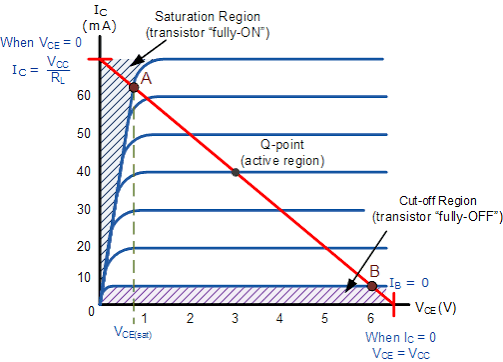
\includegraphics[width=0.8\linewidth]{figures/regiones de operacion bjt.png}
                \caption{Recta de carga y punto Q}
            \end{figure}
        \end{column}
    \end{columns}
\end{frame}

\section{Transistor de efecto de campo (FET)}

\begin{frame}
    \frametitle{Transistor de efecto de campo (FET)}
    \begin{columns}
        \begin{column}{0.4\textwidth}
            \begin{itemize}
                \item FET vs BJT
                \item Voltaje vs Corriente
                \item Unipolar vs bipolar
                \item Impedancia de entrada
                \item Puerta, drenador y fuente
            \end{itemize}
        \end{column}
        \begin{column}{0.6\textwidth}
            \begin{figure}
                \centering
                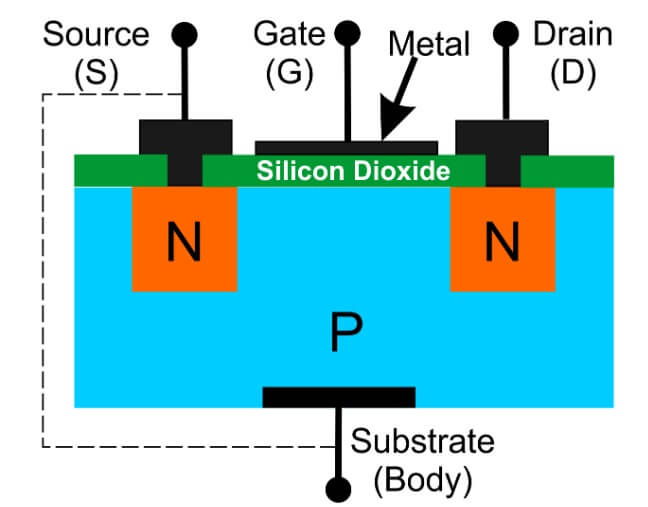
\includegraphics[width=0.8\linewidth]{figures/mosfet-cross-section.jpg}
                \caption{Diagrama de sección transversal de un FET}
            \end{figure}
        \end{column}
    \end{columns}
\end{frame}

\begin{frame}
    \frametitle{Tipos de FET}
    \begin{columns}
        \begin{column}{0.4\textwidth}
            \begin{itemize}
                \item Canal N y P
                \item JFET y MOSFET
            \end{itemize}
        \end{column}
        \begin{column}{0.6\textwidth}
            \begin{figure}
                \centering
                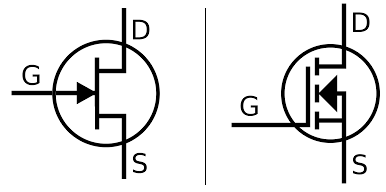
\includegraphics[width=0.8\linewidth]{figures/JFET-vs-MOSFET.png}
                \caption{JFET y MOSFET}
            \end{figure}
        \end{column}
    \end{columns}
\end{frame}

\section{Aplicaciones}

\section{Referencias}

\begin{frame}
  \frametitle{Blocks and emphasis}
  \begin{block}{Theorem}
    You can create a \texttt{block} to put emphasis in a theorem or something else.
    \begin{equation*}
      \therefore e^{i\pi} + 1 = 0
    \end{equation*}
  \end{block}

  \begin{exampleblock}{Example}
    Similarly you can create a \texttt{exampleblock} for examples or interactive exercises.
    \begin{enumerate}
      \item This is the first question
      \item this is the second questions
    \end{enumerate}
  \end{exampleblock}

  \begin{alertblock}{Alert}
    This block is used to give an alert!
  \end{alertblock}
\end{frame}


\begin{frame}
  \frametitle{Citations}
  \centering
  \begin{columns}
    \begin{column}{0.4\textwidth}
      \begin{itemize}
        \item Citations are a \textbf{must}, and should always be cited with a citation command
        \item In the current example I am using \texttt{natbib} natural science style
        \item You can include other styles such as IEEE (which only supports \texttt{cite} command)
        \item To add a citation we use the \textit{natbib} package, which is the standard way of citation in natural sciences, a citation example would be like this \citep{2022A&A...663A.106C}
      \end{itemize}
    \end{column}
    \begin{column}{0.4\textwidth}
      \begin{itemize}
        \item The \texttt{natbib} in-line citations are:
        \begin{itemize}
            \item \citep{2022A&A...663A.106C}
            \item \citet{2022A&A...663A.106C}
            \item \citep[see][]{2022A&A...663A.106C}
        \end{itemize}
        \item You can also only quote the year or name using natbib:
        \begin{itemize}
          \item \citeyear{2022AJ....163...65C}
          \item \citealt{2022AJ....163...65C}
        \end{itemize}
      \end{itemize}
    \end{column}
  \end{columns}
\end{frame}


\begin{frame}
  \frametitle{Equations and units}
  \small
  \begin{itemize}
    \item When writing equations make sure you include the name of the variable in math mode and \textbf{not} in text mode, i.e., the variable is $z$ and \textbf{not} z, \textbf{z}, or \textit{z}
    \begin{equation}
      z = \sqrt{\del{\frac{x}{a}}^2 + \del{\frac{y}{b}}^2}
    \end{equation}
    \item You can highlight an important equation with the following command \texttt{tcbhighmath}
    \begin{equation}
      \tcbhighmath{\sigma_T \equiv k_c \frac{T_\text{sys}}{\sqrt{\Delta\nu t_\text{int}}}}
    \end{equation}
    \item Para escribir unidades con un formato limpio, se puede usar texto matemático directo, por ejemplo:
    \begin{equation}
        I_\nu\del{\nu,\widehat{\mathbf{n}}, \mathbf{r}, t}\dif\nu\dif\Omega \;=\; \mathrm{W\,m^{-2}}.
        \label{eq:specific_intensity}
    \end{equation}
    \item En la ecuación~\eqref{eq:specific_intensity} se muestra la unidad en modo matemático, por ejemplo $\mathrm{W\,m^{-2}}$
    \item Un ejemplo de cantidad con unidades es $c_0 = 299\,792\,458.0\,\mathrm{m\,s^{-1}}$
    \item Las unidades se escriben con formato explícito para evitar conflictos de paquetes de LaTeX.
  \end{itemize}
\end{frame}


\begin{frame}
  \frametitle{Tables}
  \centering
  \begin{columns}
    \begin{column}{0.5\textwidth}
      \begin{itemize}
        \item You may also be possible to include a Table, just make sure it is easy to read
        \item To make nice tables we suggest the package \texttt{booktabs}
        \item As shown in side Table, this lets you add bar lines and make the tables more compact
        \item Since it is a matter of taste feel free to look for your preferred one
      \end{itemize}
    \end{column}
    \begin{column}{0.4\textwidth}
      \begin{table}[t]
        \centering
        \begin{tabular}{ccc}
            \toprule
            \textbf{A} & \textbf{B} & \textbf{C} \\ \midrule
            1 & 2 & 3 \\
            1 & 2 & 3 \\
            1 & 2 & 3 \\
            1 & 2 & 3 \\
            1 & 2 & 3 \\
            \bottomrule
        \end{tabular}
        \caption{Adding a caption}
    \end{table}
    \end{column}
  \end{columns}  
\end{frame}

\begin{frame}
  \frametitle{Ti\textit{k}z example figure}
  \vspace{-.1cm}
  \begin{columns}
    \begin{column}[]{0.57\textwidth}
      \begin{figure}
        \centering
        \begin{tikzpicture}[font=\footnotesize]
    
            \def\linethick{0.6pt}
    
            \coordinate (M1) at (-2, 0);
            \coordinate (m) at (2, 4);
            \coordinate (M2) at (4, 0);
    
            \draw[->] (-3, 0) -- (5, 0) node[left, below] {$x$};
            \draw[->] (0, -1) -- (0, 4) node[right] {$y$};
    
            \draw[line width=\linethick] (0, 0) -- node[midway,left] {$r$} (m) node[above] {$m$};
            \draw[line width=\linethick] (M1) node[above, xshift=-10] {$M_1$} -- node[midway,left] {$s_1$} (m);
            \draw[line width=\linethick] (M2) node[above, xshift=7] {$M_2$} -- node[midway,left] {$s_2$} (m);
    
            \path (M1) -- node[midway, below] {$r_1$} (0, 0);
            \path (0, 0) -- node[midway, below] {$r_2$} (M2);
    
            % Dashed lines
    
            \draw[dashed] (M1) -- ++ (0, -1);
            \draw[dashed] (M2) -- ++ (0, -1);
            \draw[|<->|] ($(M1) + (0, -1.1)$) -- node[midway,fill=white] {$a$} ($(M2) + (0, -1.1)$);
            
            \node[below] at (0.4, 0) {CM};
    
            \draw ([shift={(0, 0)}]64:0.5) arc[radius=0.5, start angle=64, end angle=0] node[above, xshift=4] {$\theta$};
    
            % balck circles
            \filldraw[black] (m) circle(0.1);
            \filldraw[black] (M1) circle(0.17);
            \filldraw[black] (M2) circle(0.13);
            \filldraw[black] (0, 0) circle(0.05);
    
        \end{tikzpicture}
        \caption{Nice diagram using Ti\textit{k}Z. Notice that the typesetting of variables is the same as the one used in \LaTeX. Variables $\theta$, $M_1$, $M_2$, have the same font and text style.}
        \label{fig:my_tikz_fig}
    \end{figure}
    \end{column}
    \begin{column}{0.43\textwidth}
      \begin{itemize}
        \item Remember to always reference all variables and labels within the figure
        \item The three body problem, with masses: $M_1, M_2,$ and $m$, etc.
        \item If you'd like to learn Ti\textit{k}z search online in \url{https://tex.stackexchange.com} there are already made examples that you can easily modify
        \item The official tutorial is here: \url{https://tikz.dev}
        \item \textbf{Warning} the learning curve for Ti\textit{k}z is super steep, but highly rewardable!
      \end{itemize}
    \end{column}
  \end{columns}

\end{frame}



\begin{frame}
  \frametitle{Conclusions}
  \begin{itemize}
    \item The summary/conclusions slide should reference all key points and takeaways of the talk
    \item End simple, with one or two conclusions
    \item Add a figure if needed
    \item Say thank you and open the door for questions
  \end{itemize}

  \vfill
  \begin{center}
    {\Large\textbf{Thank you!}}
  \end{center}

\end{frame}

\begin{frame}
    \frametitle{References}
    \footnotesize
    \bibliographystyle{bibstyle_aas}
    \bibliography{pres_template}
\end{frame}



\end{document}
